\documentclass[12pt, letterpaper]{article}
\usepackage{listings}
\usepackage{graphicx}
\usepackage{color}
\usepackage{caption}
\usepackage{subcaption}
\usepackage{hyperref}
\usepackage{fancyhdr}
\usepackage{mathrsfs}
\usepackage[margin=3cm]{geometry}
\usepackage[dvips]{epsfig}
\setlength{\parindent}{0.0in}
\setlength{\parskip}{0.05in}

\definecolor{dkgreen}{rgb}{0,0.6,0}
\definecolor{gray}{rgb}{0.5,0.5,0.5}
\definecolor{mauve}{rgb}{0.58,0,0.82}
\definecolor{deepblue}{rgb}{0,0,0.7}
\definecolor{deepred}{rgb}{0.6,0,0}
\definecolor{deepgreen}{rgb}{0,0.5,0}
\definecolor{red}{rgb}{0.9,0,0}

\newcommand\course{CS532}
\newcommand\semester{Spring 2017}
\newcommand\hwnum{1}
\newcommand\yourname{Justin Schaffner}
\newcommand\login{JASchaff}
\newenvironment{answer}[1]{\subsection*{Problem #1}}

\pagestyle{fancyplain}
\headheight 40pt
\lhead{\yourname\ (\login)\\\course\ --- \semester}
\chead{\textbf{\Large Assignment \hwnum}}
\rhead{\today}
\headsep 40pt
\lstnewenvironment{MyBash}{\lstset{language=bash, aboveskip=3mm, belowskip=3mm, showstringspaces=false, columns=flexible, basicstyle={\small\ttfamily}, numbers=none, numberstyle=\tiny\color{grey}, keywordstyle=\color{black}, commentstyle=\color{dkgreen}, stringstyle=\color{black}, breaklines=true, breakatwhitespace=true, tabsize=3}}{}
\lstnewenvironment{MyPython}{\lstset{language=Python, aboveskip=3mm, belowskip=3mm, basicstyle=\small, otherkeywords={self}, keywordstyle=\color{deepblue}, emph={MyClass,__init__}, emphstyle=\color{deepred}, stringstyle=\color{deepgreen}, commentstyle=\color{red}, frame=tb, showstringspaces=false, breaklines=true }}{}
\lstnewenvironment{MyR}{\lstset{language=R, aboveskip=3mm, belowskip=3mm, basicstyle=\small}}{}

\begin{document}

\begin{answer}{1: Twitter Crawler}
For the twitter crawler, I began the project with the Tweepy example from adilmoujahid.com. I used Python 3.5 for all of the programs for this assignment since Tweepy hasn't been updated for 3.6. Using the Tweepy library did cause some issues with implementing the twitter crawler. The library doesn't handle the extended tweets, for this reason any URIs for twitter.com or t.co were discarded. Otherwise, the script worked as advertised, and immediately began pulling tweets and storing them in a json file. \\
When it came time to parse the URIs from the tweets, there was another issue. While trying to read the file line by line, the json library wasn't recognizing the file as json format. I spent way too much time trying to figure out how to read the file, searching for solutions in formatting or how the file was being saved and tweet layout. In the end I skipped trying to find the individual tweet out of a file and decided to parse the URI out of the tweet as Twitter streamed them in. This turned out to be a much simpler solution than trying to read the file after the fact. In order to parse the text of the tweet I used a tokeniser example from \url {<https://marcobonzanini.com/2015/03/09/mining-twitter-data-with-python-part-2/>}. This worked out really well, and it will also allow me to easily expand the functionality of the class later on to pull other data from the tweet. \\
Once I started parsing the tweets, I started getting a number of "Incomplete Read" and "Connection Reset by Peer" errors. From what I was able to gather from the forums, this was due to twitter crawler not reading the tweets as fast as Twitter was delivering them. This could have been caused by a few things. The search parameters may have been too broad, causing the number of relevant tweets to be enormous. Also, by parsing the tweets as they come in, it slowed down (however infinitesimally) the ability to process them. By changing the search parameters, it didn't completely make the problem go away, but it did allow the crawler to run for a while before it backed up, rather than after a few minutes. The only drawback is if there are too many failed connections within a certain time window, Twitter apparently blocks any new attempts for a period. This is solved by regenerating the tokens, but its not very practical. Thats one reason I let it close out rather than have it just keep reconnecting when it errors. I also noticed that if the search parameters were too narrow, eventually twitter crawler would stop getting unique URIs related to that topic. At one point I had exactly 750 URIs and I kept running the twitter crawler and getting nothing new. I suppose even with the thousands of tweets, there are only so many sources people tweet about. At that point I began changing the search parameters every couple of runs to keep getting new links. An upgrade to this would allow search parameters to be entered through the command line. Not that fancy yet.  Right now the program is called and piped to a file using the following command:\\
\begin{MyBash}
$ python3.5 Twitter_crawler.py >>twitter_links.txt
\end{MyBash}
Here is the code for the twitter crawler:\\
\begin{MyPython}
from tweepy.streaming import StreamListener
from tweepy import OAuthHandler
from tweepy import Stream
import json
import re as regex
import requests

#Variables that contains the user credentials to access Twitter API 
access_token = "826264224838057986-p2cjKY6P4qKUUbTRtDZDicIHFxXkCdu"
access_token_secret = "yTAtL6R0rb35p49qcharmzWMz5X4vQsT0Jrm2UQR7Nipf"
consumer_key = "1qH36csH37Oa1LKjgDijsxGVX"
consumer_secret = "QlVfb24OuyOGsMmF8ojWZs1N2p1eeT8ib2CK4ovntk1tpSLIaW"



class StdOutListenerParser(StreamListener):
    
    counter=0
    
    emoticons_str = r"""(?: [:=;] [oO\-]? [D\)\]\(\]/\\OpP] )"""
    regex_str = [r'<[^>]+>', r'(?:@[\w_]+)', r"(?:\#+[\w_]+[\w\'_\-]*[\w_]+)", r'http[s]?://(?:[a-z]|[0-9]|[$-_@.&amp;+]|[!*\(\),]|(?:%[0-9a-f][0-9a-f]))+', r'(?:(?:\d+,?)+(?:\.?\d+)?)', r"(?:[a-z][a-z'\-_]+[a-z])", r'(?:[\w_]+)', r'(?:\S)' ]
        
    tokens_re = regex.compile(r'('+'|'.join(regex_str)+')', regex.VERBOSE | regex.IGNORECASE)
    emoticon_re = regex.compile(r'^'+emoticons_str+'$', regex.VERBOSE | regex.IGNORECASE)
    def tokenize(self, s):
        return self.tokens_re.findall(s)
     
    def preprocess(self, s, lowercase=False):
        tokens = self.tokenize(s)
        if lowercase:
            tokens = [token if emoticon_re.search(token) else token.lower() for token in tokens]
        return tokens
    def pull_uri(self, tokens):
        linklist=[]
        for i in tokens:
            if 'http' not in i:
                continue
            try:
                tpage=requests.get(i,allow_redirects=True, stream=True)
                turl=tpage.url
                if not turl.startswith('https://twitter.com') and not turl.startswith('https://t.co'):
                    linklist.append(turl)
            except Exception:
                pass
        for i in linklist:
            print (i)
            self.counter+=1
        
    def on_data(self, data):
        tweet=json.loads(data)
        if 'text' in tweet:
            tokens=self.preprocess(tweet['text'])
            self.pull_uri(tokens)
        if self.counter==2000:
            return False
        return True

    def on_error(self, status_code):
        print (status_code)
        if status_code==420:
            return False

if __name__ == '__main__':

    #This handles Twitter authetification and the connection to Twitter Streaming API
    l = StdOutListenerParser()
    auth = OAuthHandler(consumer_key, consumer_secret)
    auth.set_access_token(access_token, access_token_secret)
    stream = Stream(auth, l)

    #This line filters Twitter Streams to capture data by keywords
    stream.filter(track=['immigrant http, Bowling Green http'])
    
\end{MyPython}
In order to sort out unique links I created a class Unique Set with the output file from Twitter Crawler as the only command line argument:\\
\begin{MyBash}
$ python3.5 Unique_Set.py twitter_links.txt
\end{MyBash}
Here is the code for Unique Set:
\begin{MyPython}
from sys import argv

class Unique_Set():
    
    def unique_filter(self, this_list):
        newset=set()
        for i in this_list:
            newset.add(i)
        return newset
#this pulls a filename from the command line and processes it, saving it back to the same file and overwriting it
if __name__ == '__main__':
    u=Unique_Set()
    filename=argv[1]
    with open(filename, 'r+') as file:
        file_list=[]
        for line in file:
            file_list.append(line)
        print(len(file_list))
        newset=u.unique_filter(file_list)
        file_list=list(newset)
        print (len(file_list))
        file.seek(0)
        for i in file_list:
            file.write(i)
        file.truncate()

\end{MyPython}

\end{answer}

\begin{answer}{2-3: Time Maps and Carbon Dating}
Get Mementos takes the list of URIs from Twitter Crawler after it has been filtered with Unique Set and plugs them into ODU's memento aggregator, then counts the returned mementos. If there are mementos, then the URI is also forwarded to the Carbon Date tool. The data collected is then stored in "data\textunderscore set.txt" as a tabulated file. The first column is the number of mementos and the second is the estimated age in days. For this implementation, Carbon Date, available at  \url {https://github.com/oduwsdl/CarbonDate} was run as a local server in Docker.\\
Once I pulled the data, I ran it through r to get the following histogram showing the number of Momentos per URI:\\
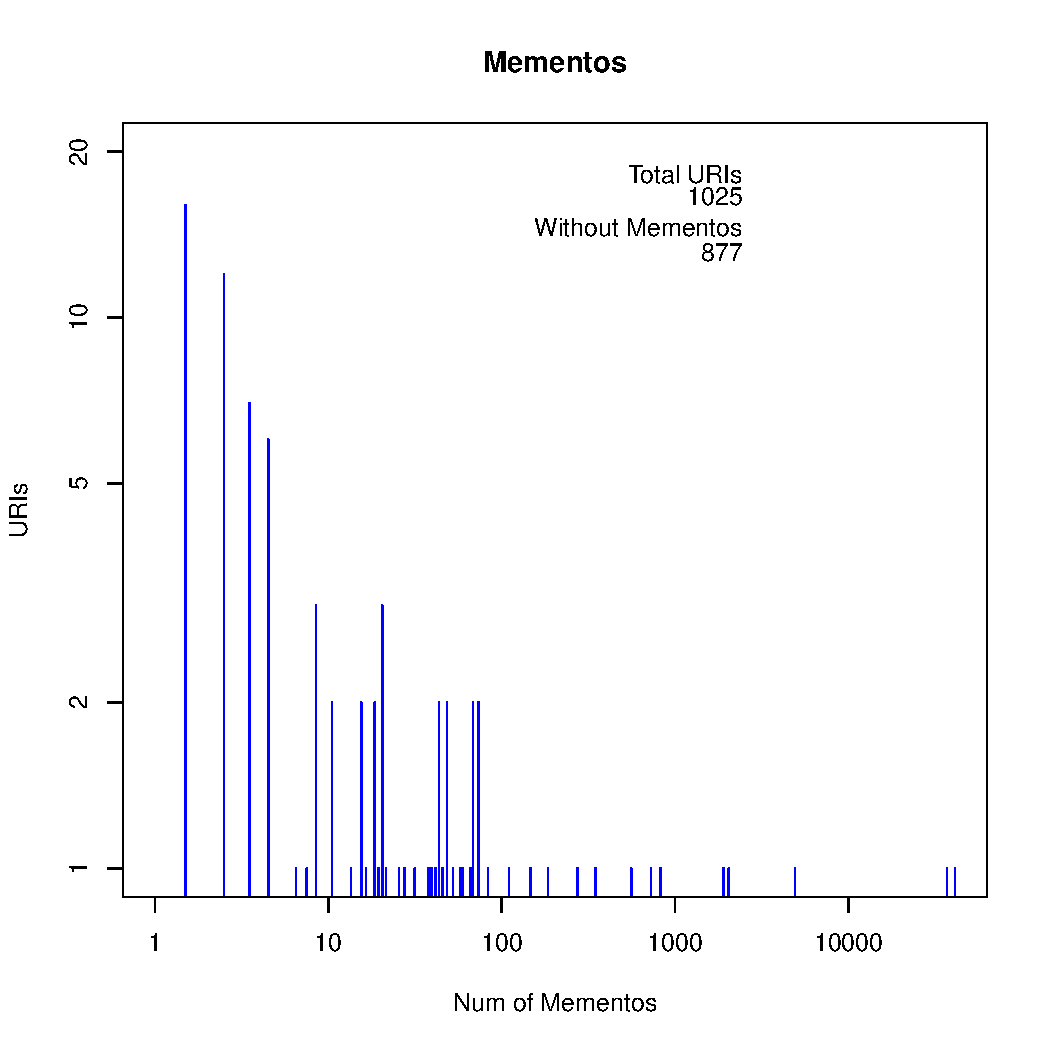
\includegraphics[width=\linewidth]{mem_data}
Here is the R code I used to generate the graphic.
\begin{MyR}
require(graphics)
pdf("Desktop/mem_data.pdf")
data_table<-read.table(file="Desktop/data_set.txt", header=T, sep="\t")
mem_data<-c(data_table$mem)
max_mem<-max(mem_data)
num_zero_mem<- length(mem_data[mem_data==0])
h<-hist(mem_data, plot=F, breaks=max_mem)
plot(h$mids, h$counts, log='xy', xlim= c(1, max_mem), ylim=c(1,20), pch=20, col='blue', main="Mementos", xlab="Num of Mementos", ylab="Frequency", type='h')
text(c(3000,3000,3000,3000),c(18,16.4,14.4,13), labels=c("Total URIs", length(mem_data), "Without Momentos", num_zero_mem), pos=2, col='black')
dev.off()
\end{MyR}
I then used both columns of data to get the number of Mementos vs the Age of the URI in days:\\
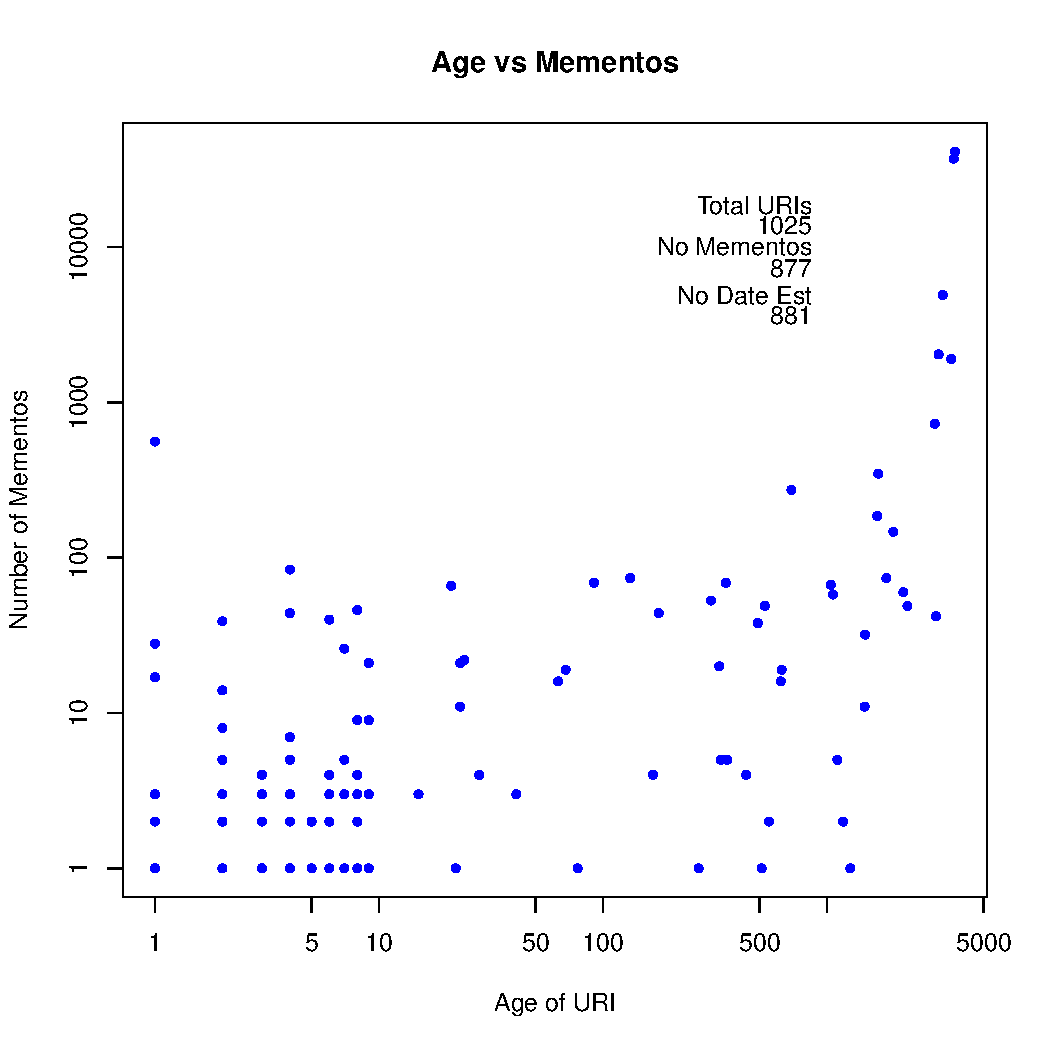
\includegraphics[width=\linewidth]{age_data}
\\
Here is the R code used to generate the graphic.
\begin{MyR}
require(graphics)
pdf("Desktop/age_data.pdf")
data_table<-read.table(file="Desktop/data_set.txt", header=T, sep="\t")
num_na<-length(data_table$age[data_table$age=='NA'])
num_uri<-length(data_table$mem)
num_zero_mem<- length(data_table$mem[data_table$mem==0])
data<-data_table[!data_table$mem=='0' & !data_table$age=='NA',]
max_age<-max(data$age)
max_mem<-max(data$mem)
plot(data$age, data$mem, log="xy", pch=20, col='blue', main="Age vs Mementos", xlab="Age of URI", ylab="Number of Mementos", type='p' )
text(c(1000,1000,1000,1000,1000,1000),c(18000,13300,9750,7000,4700,3500), labels=c("Total URIs", num_uri, "No Mementos", num_zero_mem, "No Date Est", num_na), pos=2, col='black')
dev.off()
\end{MyR}
This is the code for Get Mementos:
\begin{MyPython}
import requests
import re
from sys import argv
from urllib.parse import urljoin
from datetime import datetime
import json


class get_mementos():
  
    def get_aggregate(self, uri):
        aggregate='http://memgator.cs.odu.edu/timemap/link/'.rstrip()
        uri=aggregate+uri.rstrip()
        tbody=requests.get(uri)
        print(tbody.status_code)
        if not(tbody.status_code == 200):
                raise StopIteration
        for line in tbody:
                yield line
        
    def get_age(self, uri):
        agelink='http://localhost:8888/cd?url='.rstrip()
        uri=agelink+uri.rstrip()
        r=requests.get(uri)
        data=json.loads(r.text)
        date_string=data['Estimated Creation Date']
        cdate=datetime.strptime(date_string, '%Y-%m-%dT%H:%M:%S')
        return (datetime.now()-cdate).days
        
    def get_data(self, uri):
        num_mementos=0
        age=0
        for line in self.get_aggregate(uri):
            if b'memento' in line:
                num_mementos+=1
                    
        if num_mementos>0:
            age=self.get_age(uri)
            return(num_mementos, age)
        return (num_mementos, 'NA')



if __name__ == '__main__':
    filename=argv[1]
    r=get_mementos()
    with open("data_set.txt", 'w') as outfile:    
        with open(filename, 'r') as file:
            for line in file:
                #print(line)
                print('\t'.join(str(v) for v in r.get_data(line)), file=outfile)

\end{MyPython}
\end{answer}


\end{document}